\chapter{Processamento/Tratamento de Dados}

Nesta etapa, nosso principal objetivo foi compatibilizar as imagens capturadas por diferentes sensores para construir uma série temporal de imagens de satélite pronta para análise, conhecida como \textit{Analysis Ready Data - ARD}. 

\section{Compatibilização dos sensores}

Para gerarmos uma série temporal de imagens de satélite providas de diferentes sensores, uma das primeiras etapas que devemos realizar é a compatibilização dos valores de reflectância considerando as características espectrais dos diferentes sensores. Neste trabalho, utilizamos imagens obtidas pelo sensor Operational Land Imager (OLI), acoplado no satélite Landsat 8, e pelo sensor Multispectral Instrument (MSI) acoplado nos satélites Sentinel 2A e 2B. Para compatibilizar as imagens dos diferentes sensores, utilizamos um método de ajuste de histograma linear. O método de ajuste de histograma linear é um método simplificado que permite reescalonar os valores dos \textit{pixels} de uma imagem de forma que eles fiquem mais próximos do valor dos \textit{pixels} de uma imagem de referência. Para aplicar este método, calculamos a média e o desvio padrão da imagem de referência e da imagem que queremos ajustar para encontrarmos os coeficientes de \textit{gain} e \textit{offset}, por banda, que deveremos utilizar na função abaixo para realizar o ajuste das imagens. 

\begin{equation}
banda\_ajustada = banda\_original * gain + offset,
\end{equation} \\ onde  $gain=  \frac{S}{si} $ e $offset = \overline{X} - \overline{xi}$, com $S$ = desvio padrão da banda de referência, $si$ = desvio padrão da banda original, $ \overline{X}$ = média da banda de referência e $\overline{xi}$ = média da banda original. 

Na Tabela \ref{tab:coeficientes_ajuste_histograma} apresentamos o conjunto de coeficientes que utilizamos para ajustar todas as imagens Sentinel 2A e 2B utilizadas neste trabalho e deixá-las com o valor dos \textit{pixels} mais próximo do obtido nas imagens Landsat 8.   

\begin{table}[H]
\caption{Coeficientes de regressão linear usados para ajustar as imagens Sentinel 2A e 2B, sensor MSI, para torná-las compatíveis com as imagens Landsat 8, sensor OLI.}
\label{tab:coeficientes_ajuste_histograma}
\centering
\begin{adjustbox}{width=0.5\textwidth}
\begin{tabular}{lll|l|l|}
\cline{4-5}
                                         &                                         &                    & \multicolumn{2}{c|}{\textbf{Sensor MSI}} \\ \hline
\multicolumn{1}{|l|}{\textbf{Banda ARD}} & \multicolumn{1}{l|}{\textbf{Banda OLI}} & \textbf{Banda MSI} & \textbf{\textit{Gain}}     & \textbf{\textit{Offset}}     \\ \hline
\multicolumn{1}{|l|}{BLUE}               & \multicolumn{1}{l|}{2}                  & 2                  & 1,0443             & -0,0644             \\ \hline
\multicolumn{1}{|l|}{GREEN}              & \multicolumn{1}{l|}{3}                  & 3                  & 1,1553             & -0,0388             \\ \hline
\multicolumn{1}{|l|}{RED}                & \multicolumn{1}{l|}{4}                  & 4                  & 1,0278             & -0,0200             \\ \hline
\multicolumn{1}{|l|}{NIR}                & \multicolumn{1}{l|}{5}                  & 8                  & 1,1393             & -0,0054             \\ \hline
\multicolumn{1}{|l|}{SWIR1}              & \multicolumn{1}{l|}{6}                  & 11                 & 1,0257             & -0,0067             \\ \hline
\multicolumn{1}{|l|}{SWIR2}              & \multicolumn{1}{l|}{7}                  & 12                 & 1,0514             & -0,0078             \\ \hline
\end{tabular}
\end{adjustbox}
\end{table}

Ao aplicarmos a correção em todas as imagens Sentinel 2A/2B em uma série temporal (Figura \ref{fig:serie_temporal_corrigida}) é possível constatarmos que, após a correção, as imagens Sentinel 2, que antes estavam com um índice de vegetação NDVI, que utilizou as bandas NIR e red, com valores mais baixos que as imagens Landsat 8, passaram a ficar com os valores de NDVI mais próximos dos valores obtidos no Landsat 8, formando, assim, uma série única e consistente ("Série Ajustada") com imagens dos dois sensores.     

\begin{figure}[H]
\centering
\caption{Exemplo do efeito da compatibilização entre os sensores para um ponto localizado nas coordenadas -45,739364 e -12,156442 (lon, lat) para o período de 01/10/2019 à 01/10/2020.}
\label{fig:serie_temporal_corrigida}
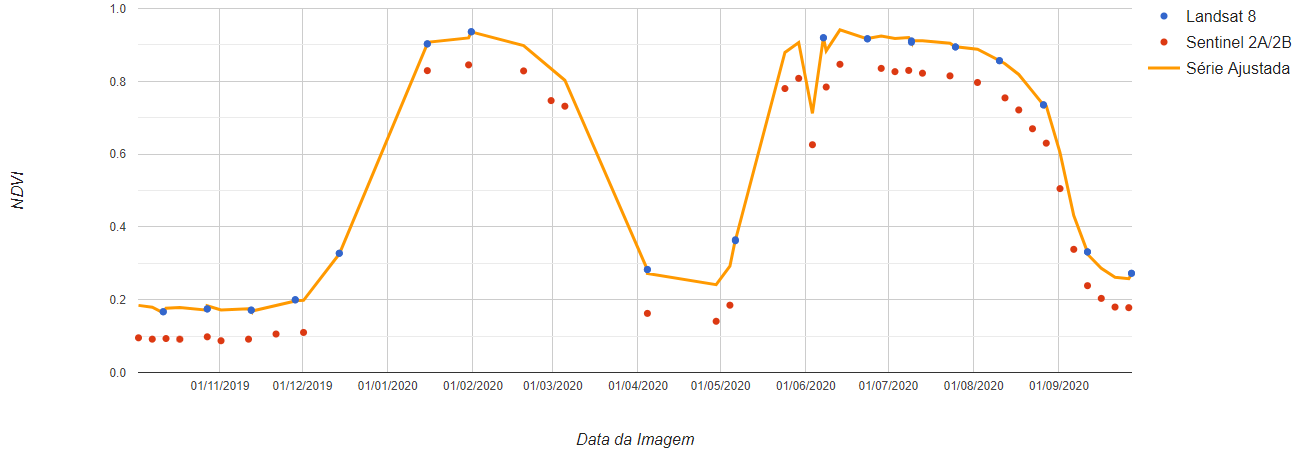
\includegraphics[width=0.7\textwidth]{figuras/serie_temporal_ajustada.png}
\label{fig:correcao_brdf}
\end{figure}


\section{Função de distribuição de reflectância bidirecional}

As imagens adquiridas através de sensores ópticos são suscetíveis as variações dos ângulos (zenital e azimutal) do Sol no momento da captura da imagem, assim como também ao próprio ângulo de visada do sensor, que podem gerar alteração no sombreamento da vegetação e superfície do solo e comprometer a qualidade final da imagem \cite{hadjimitsis2010atmospheric}. A correção dessa interferência na captura da imagem pode ser feita a partir da técnica de BRDF (\textit{Bidirectional Reflectance Distribution Function}) \cite{schaaf2002first}. Neste trabalho, aplicamos esta correção nas imagens utilizando a abordagem proposta por \citeonline{roy2016general}. Na Figura \ref{fig:correcao_brdf} apresentamos o efeito da correção BRDF aplicada em duas imagens que apresentam o efeito da iluminação do sol. 

\begin{figure}[H]
\caption{Efeito da correção da iluminação utilizando a função de distribuição de reflectância bidirecional - BRDF (b) aplicado nas imagens LC08\_178059\_20160130 e LC08\_179059\_20160206 originais (a) adquiridas pelo satélite Landsat 8, sensor OLI, na composição falsa cor (NIR, SWIR1, red).}
\label{fig:correcao_brdf}
\centering
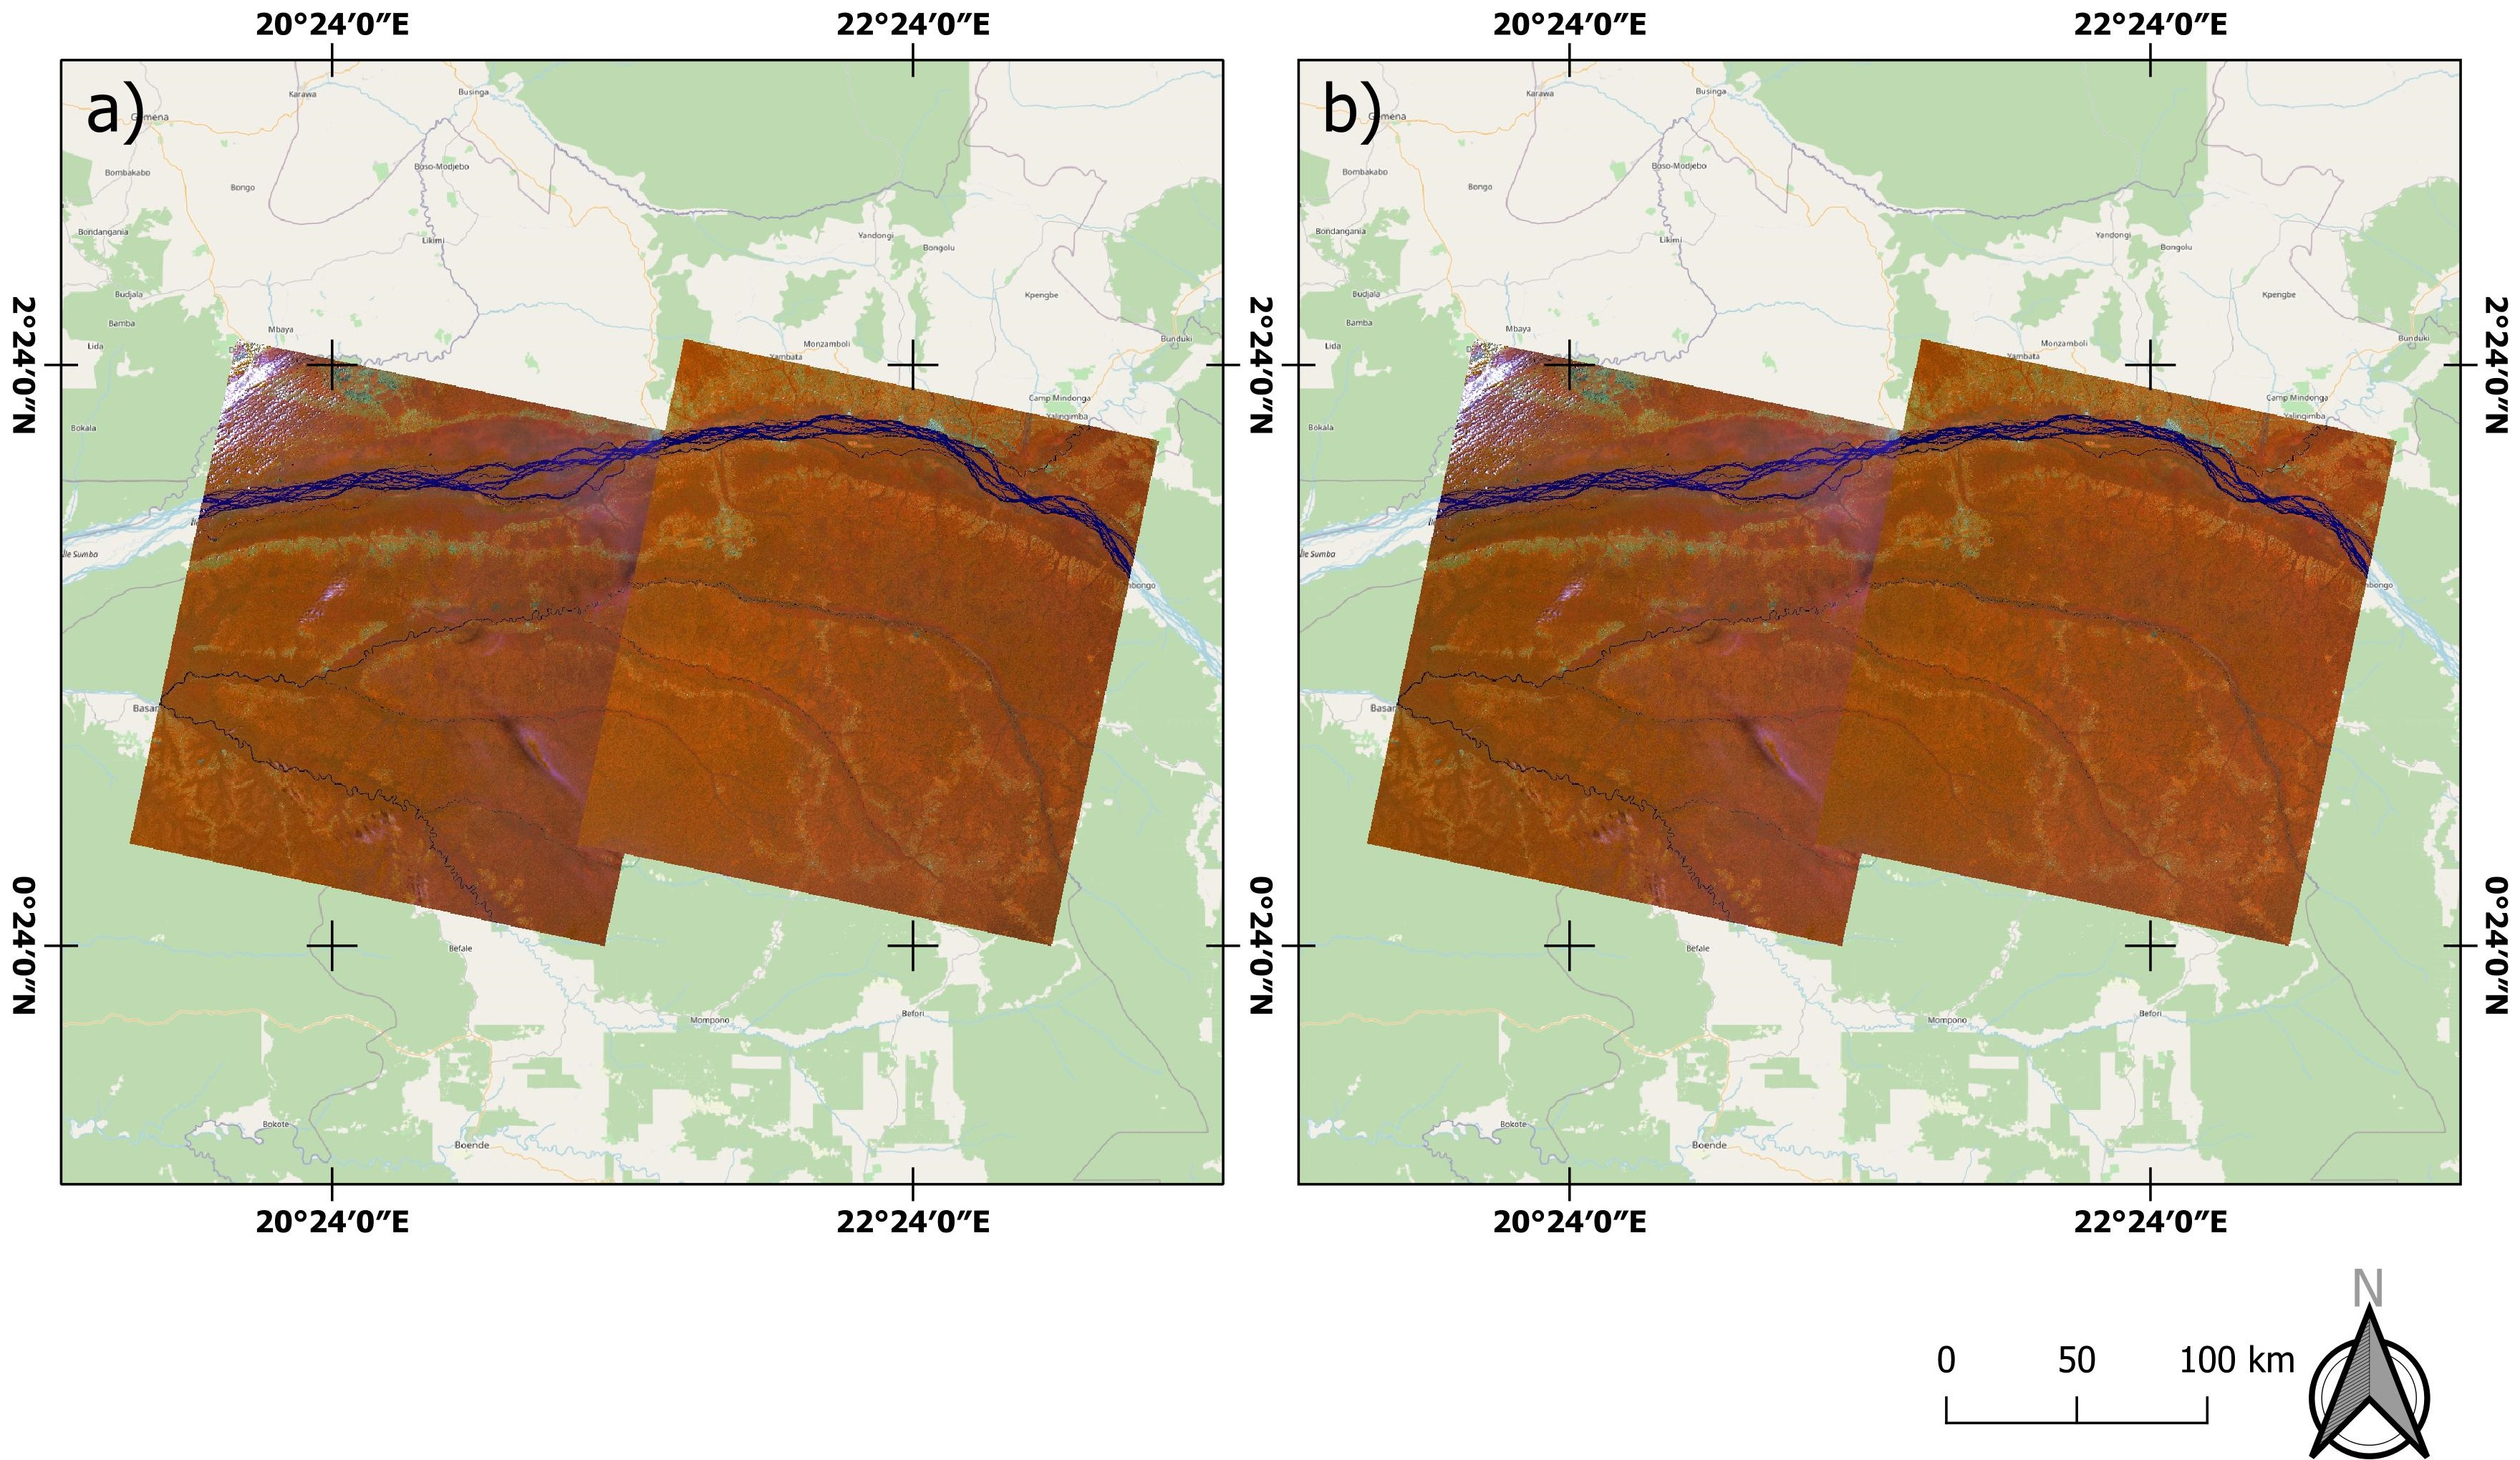
\includegraphics[width=0.6\textwidth]{figuras/aplicacao_brdf.jpg}
\end{figure}

\section{Iluminação do Terreno}

Além do efeito provocado pela variação dos ângulos do sol e do ângulo de visada do sensor, explicados na seção anterior, há também variações de iluminação provocadas pela topografia do terreno, que podem alterar o valor de reflectância do \textit{pixel}, efeito que pode se acentuar com a baixa elevação do sol e superfícies mais ásperas, como montanhas e áreas com alta declividade. 

Para realizarmos a correção da iluminação do terreno, utilizamos a implementação feita por \citeonline{poortinga2019mapping} baseada na abordagem proposta por \citeonline{soenen2005scs}. Nesta correção, utilizamos o modelo digital de elevação, produzido pela \textit{Shuttle Radar Topography Mission} - SRTM \cite{farr2007shuttle}, para obter a declividade e o aspecto da superfície do terreno e os valores contidos nos metadados da imagem referentes aos ângulos zenital e azimutal do sol no momento da captura da imagem. A Figura \ref{fig:correcao_iluminacao_terrano} apresenta um exemplo do efeito da correção em uma imagem de satélite. 

\begin{figure}[H]
\caption{Efeito da correção da iluminação do terreno (b)  aplicado em um recorte da imagem S2A\_MSIL1C\_20210703T132241\_N0301\_R038\_T23LLF\_20210703T164601 (a) adquirida pelo satélite Sentinel 2A, sensor MSI, na composição falsa cor (NIR, SWIR1, RED)}
\label{fig:correcao_iluminacao_terrano}
\centering
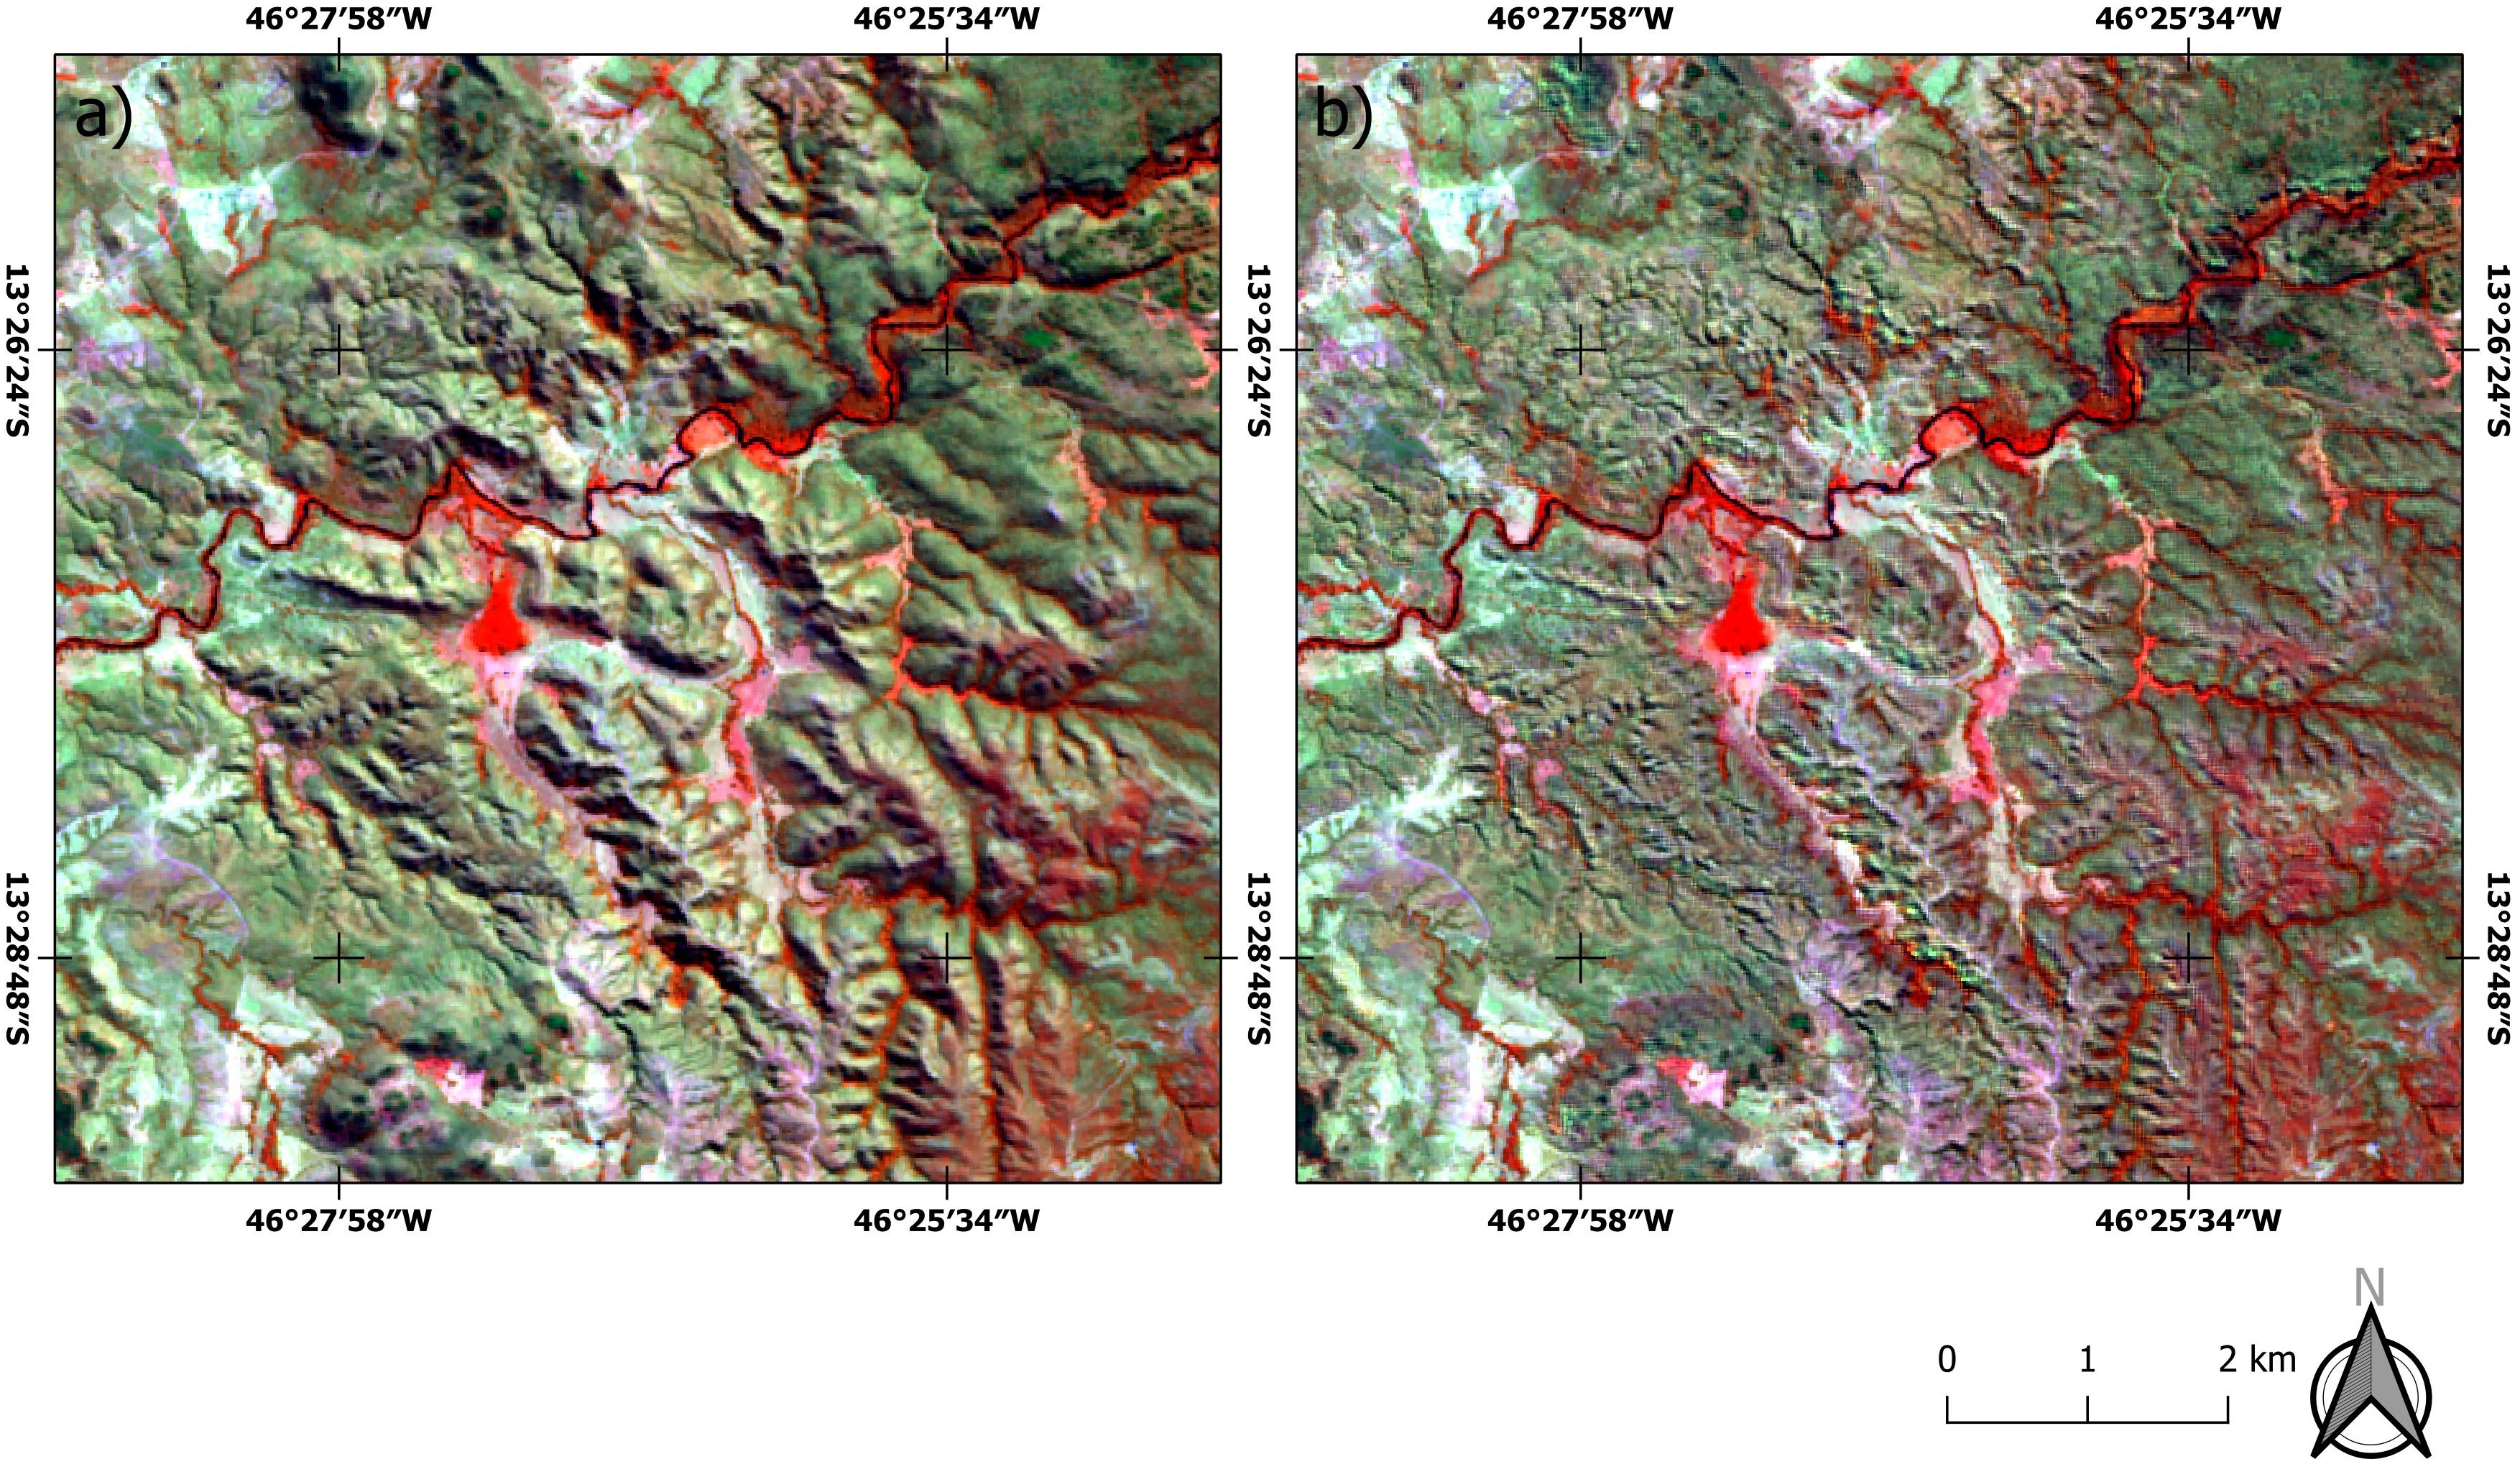
\includegraphics[width=0.6\textwidth]{figuras/aplicacao_correcao_terreno.jpg}
\end{figure}

\section{Máscara de nuvens e sombra de nuvens}

Nuvens e sombra de nuvens podem afetar significativamente sensores ópticos como Landsat 8 OLI e Sentinel 2 MSI,  pois obstruem a visão do sensor e impedem que seja possível visualizar, nas imagens, os alvos em campo como a vegetação, agricultura, pastagem e etc. Dito isso, uma das etapas que realizamos no tratamento das imagens foi remover as nuvens e sombra de nuvens das imagens e deixar apenas \textit{pixels} livres de nuvens e sombra de nuvens (Figura \ref{fig:remocao_nuvens}).  

Para remover as nuvens e sombra de nuvem no Landsat 8, utilizamos a banda de qualidade (QA\_pixel) presente nas imagens de satélite. A banda de qualidade contém estatísticas de qualidade coletadas dos dados da imagem e informações da máscara de nuvem para cada imagem. As imagens dos satélites Sentinel 2A e 2B também possuem uma banda de qualidade indicando os \textit{pixels} de nuvens, porém com uma qualidade muito inferir a banda de qualidade disponível no Landsat 8. A qualidade inferior na detecção de nuvens dos satélites Sentinel 2A e 2B se deve ao fato de que o sensor MSI, presente nos dois satélites, não possui a capacidade de capturar na faixa do infravermelho de ondas longas, também conhecido como banda de temperatura ou banda do termal, essencial para a detecção de nuvens e sombra de nuvens. Como alternativa à banda de qualidade, a ESA lançou uma coleção de imagens que contem, para cada imagem Sentinel 2A/2B, uma imagem com uma única banda em cada \textit{pixel} representa a probabilidade, de 0 à 100, daquele pixel ser nuvem na imagem do satélite original. Essa coleção extra com essas máscaras de probabilidade de nuvem utilizam o algoritmo \textit{s2cloudless} \cite{zupancimproving}. 

\begin{figure}[H]
\caption{Exemplo do processo de identificação de nuvens e sombra de nuvens (áreas amarelas em (b) ) e sua remoção das imagens (áreas com dado nulos, ou cor branca, em (c) ) aplicado em um recorte da imagem LC08\_220069\_20210101 (a) adquirida pelo satélite Landsat 8, sensor OLI, na composição falsa cor (NIR, SWIR1, red).}
\label{fig:remocao_nuvens}
\centering
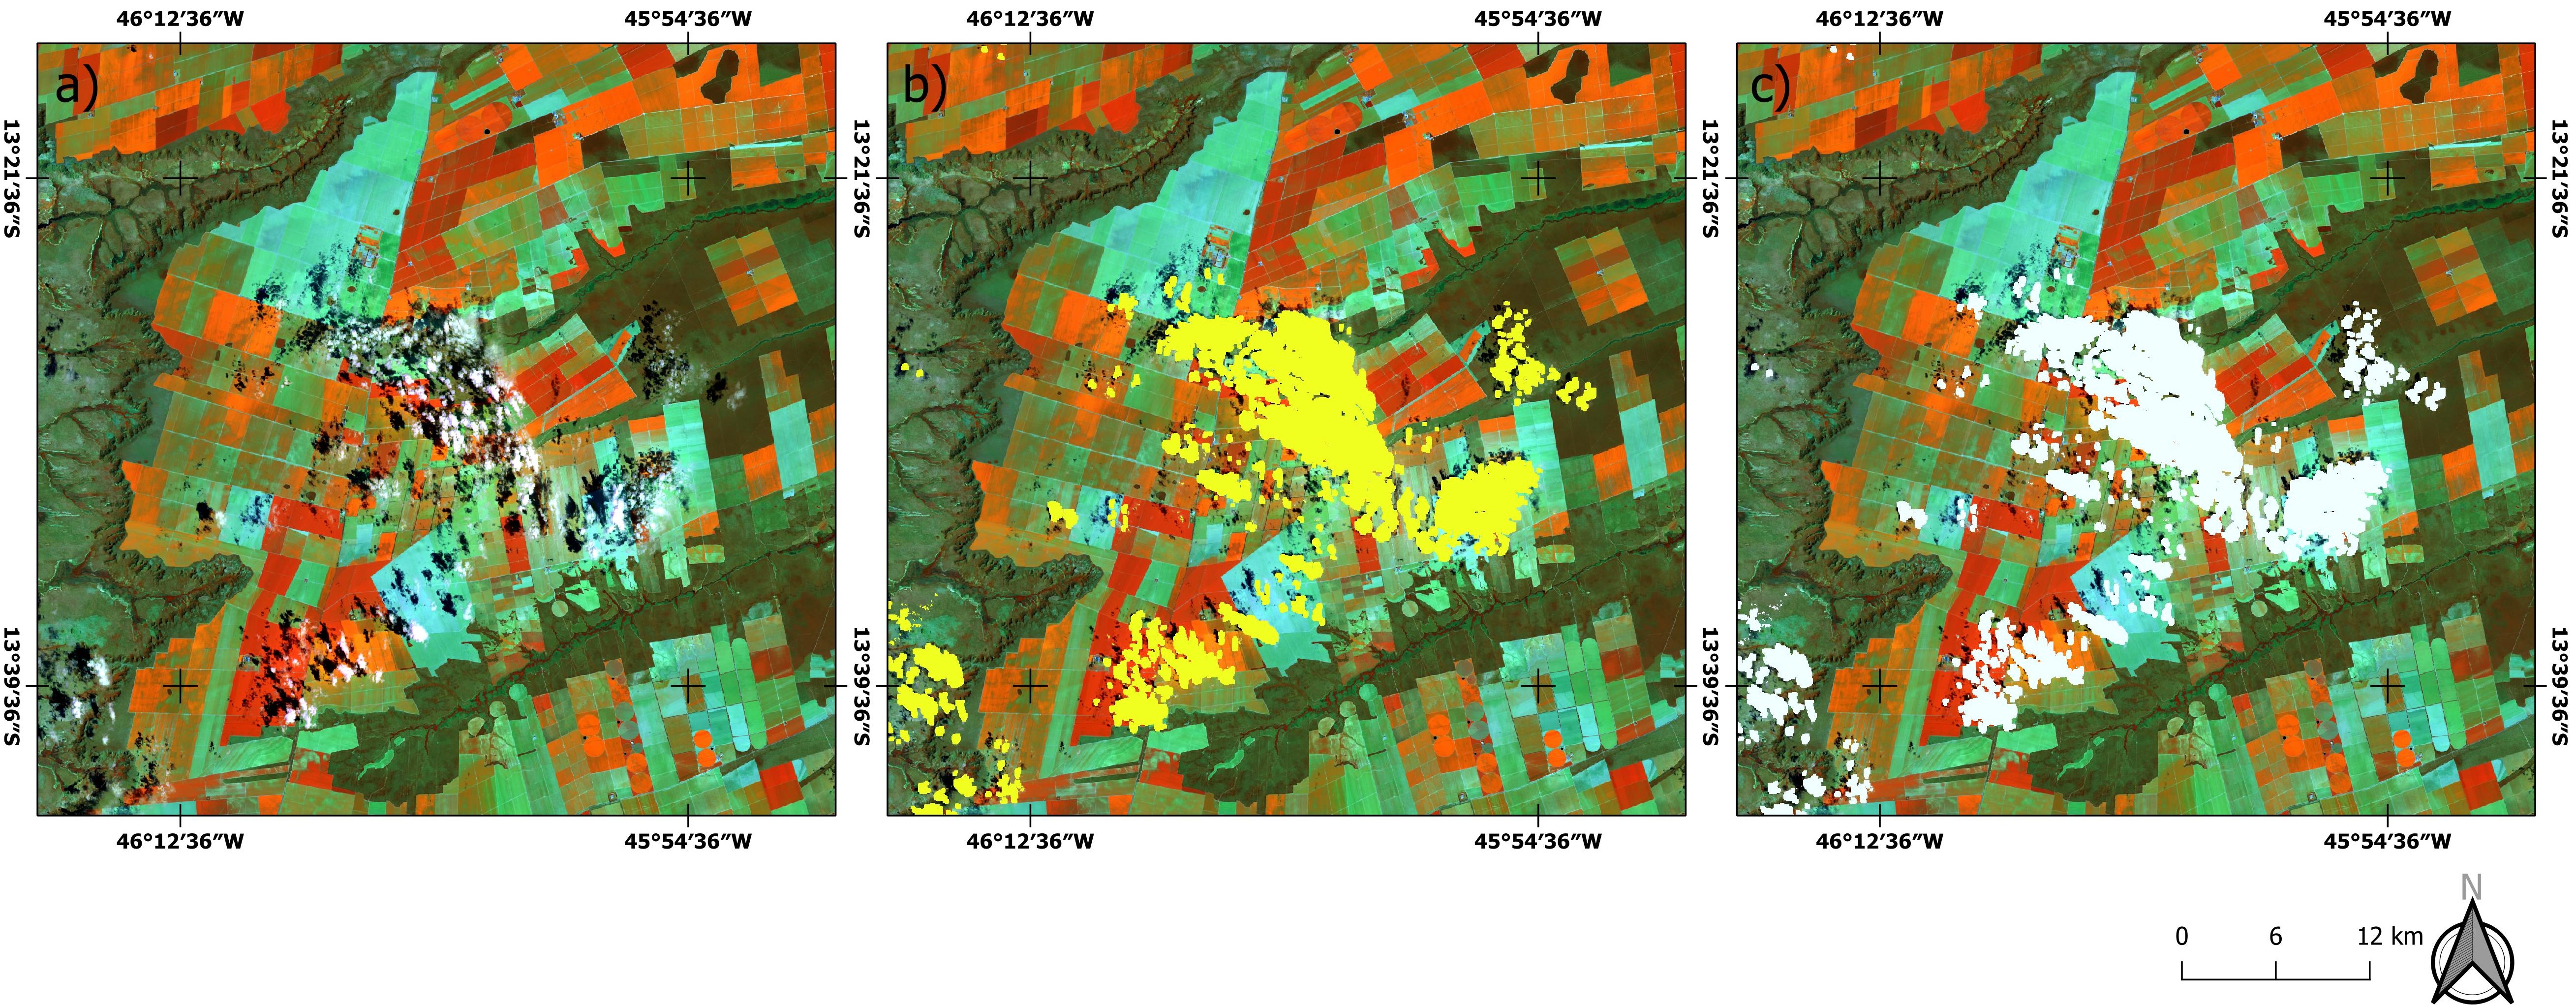
\includegraphics[width=0.8\textwidth]{figuras/mascara_nuvens.jpg}
\end{figure}

\section{Suavização das séries temporais}
\label{sec:suavizacao_series_temporais}

Mesmo com o processo de remoção de nuvens e sombra de nuvens que foi aplicado nas imagens, ainda é possível que existam resquícios de nuvens e sombra de nuvens que não foram apagadas e isso pode afetar os valores de reflectâncias das bandas das imagens e índices de vegetação utilizados. Para diminuir o efeito desses ruídos, aplicamos uma média móvel considerando a junção das duas coleções de imagens, Landsat 8 e Sentinel 2A/2B, e uma janela móvel com tamanho de 16 dias (Figura \ref{fig:serie_ajustada_com_media_movel}).

\begin{figure}[H]
\caption{Exemplo do efeito da suavização da série temporal para um ponto localizado nas coordenadas -45,739369 e -12,156452 (lon, lat) para o período de 01/10/2019 à 01/10/2020. }
\label{fig:serie_ajustada_com_media_movel}
\centering
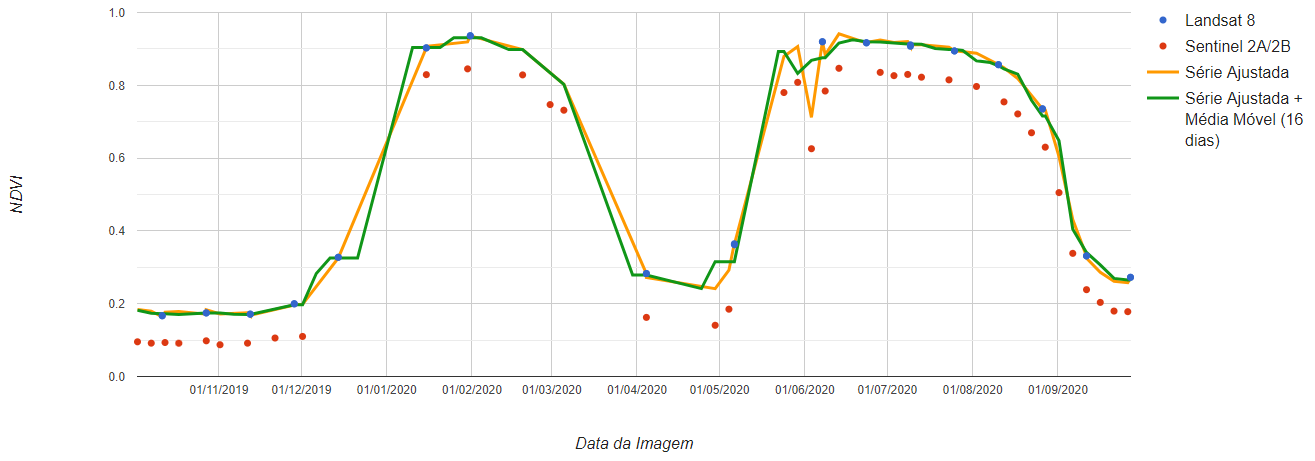
\includegraphics[width=0.7\textwidth]{figuras/serie_temporal_ajustada_media_movel.png}
\end{figure}

\section{Geração dos produtos a cada 16 dias}

A etapa final do processamento das imagens foi uma agregação temporal das imagens individuais em composições de 16 dias. O intervalo de composição foi selecionado correspondente aos produtos de dados MODIS Nível 3. O uso de um intervalo de 16 dias reduz o requisitos para download, armazenamento e processamento de dados em comparação com as imagens individuais que podem ter uma cadência de até 3 dias. Ao longo do ano, foram gerados 23 produtos que foram utilizados para o treinamento e classificação dos modelos. % (Tabela \ref{tab:produtos_16_dias}).

% \begin{table}[H]
% \caption{Dia do ano (DOY) de início e fim para os intervalos de composição dos produtos de 16 dias.}
% \label{tab:produtos_16_dias}
% \centering
% \begin{adjustbox}{width=0.5\textwidth}
% \begin{tabular}{|l|l|l|llll}
% \cline{1-3} \cline{5-7}
% \textbf{Id produto} & \textbf{DOY inicial} & \textbf{DOY final} & \multicolumn{1}{l|}{} & \multicolumn{1}{l|}{\textbf{Id produto}} & \multicolumn{1}{l|}{\textbf{DOY inicial}} & \multicolumn{1}{l|}{\textbf{DOY final}} \\ \cline{1-3} \cline{5-7} 
% 1                   & 1                           & 16                        & \multicolumn{1}{l|}{} & \multicolumn{1}{l|}{13}                  & \multicolumn{1}{l|}{193}                         & \multicolumn{1}{l|}{208}                       \\ \cline{1-3} \cline{5-7} 
% 2                   & 17                          & 32                        & \multicolumn{1}{l|}{} & \multicolumn{1}{l|}{14}                  & \multicolumn{1}{l|}{209}                         & \multicolumn{1}{l|}{224}                       \\ \cline{1-3} \cline{5-7} 
% 3                   & 33                          & 48                        & \multicolumn{1}{l|}{} & \multicolumn{1}{l|}{15}                  & \multicolumn{1}{l|}{225}                         & \multicolumn{1}{l|}{240}                       \\ \cline{1-3} \cline{5-7} 
% 4                   & 49                          & 64                        & \multicolumn{1}{l|}{} & \multicolumn{1}{l|}{16}                  & \multicolumn{1}{l|}{241}                         & \multicolumn{1}{l|}{256}                       \\ \cline{1-3} \cline{5-7} 
% 5                   & 65                          & 80                        & \multicolumn{1}{l|}{} & \multicolumn{1}{l|}{17}                  & \multicolumn{1}{l|}{257}                         & \multicolumn{1}{l|}{272}                       \\ \cline{1-3} \cline{5-7} 
% 6                   & 81                          & 96                        & \multicolumn{1}{l|}{} & \multicolumn{1}{l|}{18}                  & \multicolumn{1}{l|}{273}                         & \multicolumn{1}{l|}{288}                       \\ \cline{1-3} \cline{5-7} 
% 7                   & 97                          & 112                       & \multicolumn{1}{l|}{} & \multicolumn{1}{l|}{19}                  & \multicolumn{1}{l|}{289}                         & \multicolumn{1}{l|}{304}                       \\ \cline{1-3} \cline{5-7} 
% 8                   & 113                         & 128                       & \multicolumn{1}{l|}{} & \multicolumn{1}{l|}{20}                  & \multicolumn{1}{l|}{305}                         & \multicolumn{1}{l|}{320}                       \\ \cline{1-3} \cline{5-7} 
% 9                   & 129                         & 144                       & \multicolumn{1}{l|}{} & \multicolumn{1}{l|}{21}                  & \multicolumn{1}{l|}{321}                         & \multicolumn{1}{l|}{336}                       \\ \cline{1-3} \cline{5-7} 
% 10                  & 145                         & 160                       & \multicolumn{1}{l|}{} & \multicolumn{1}{l|}{22}                  & \multicolumn{1}{l|}{337}                         & \multicolumn{1}{l|}{352}                       \\ \cline{1-3} \cline{5-7} 
% 11                  & 161                         & 176                       & \multicolumn{1}{l|}{} & \multicolumn{1}{l|}{23}                  & \multicolumn{1}{l|}{353}                         & \multicolumn{1}{l|}{365 (366)}                 \\ \cline{1-3} \cline{5-7} 
% 12                  & 177                         & 192                       &                       &                                          &                                                  &                                                \\ \cline{1-3}
% \end{tabular}
% \end{adjustbox}
% \end{table}

\section{Padronização das classes utilizadas para o treinamento dos modelos}

Os polígonos disponíveis nos dados de referência foram coletados em trabalhos de campo e contém um conjunto de classes de uso e cobertura da terra que foram definidos pelos analistas. Das classes definidas, algumas possuem poucas amostras, enquanto outras possuem uma definição de classe que não compreende uma categoria de uso e cobertura da terra, como a classe "not identified". Neste trabalho, focamos nossos esforços no desenvolvimento de uma metodologia de mapeamento do uso e cobertura da terra que busca mapear as classes mais representativas e consistentes do conjunto de dados original. Para isso, removemos e agregamos algumas classes disponíveis no conjunto original e geramos um novo conjunto com treze classes de uso e cobertura (Tabela \ref{tab:classes_remapeadas}) que possui as classes mais representativas e consistentes do conjunto de dados original. 

% https://code.earthengine.google.com/bbc8502f24f5b562213c9cac88444bec

\definecolor{soybean}{rgb}{255, 227, 46}

\begin{table}[H]
\caption{Classes originais presentes nos dados de referência e sua classe correspondente na nova legenda que foi criada para simplificar a lista de classes que foram mapeadas neste trabalho.}
\label{tab:classes_remapeadas}
\centering
\begin{adjustbox}{width=0.5\textwidth}
\begin{tabular}{|l|l|l|l|l|}
\hline
\textbf{Classe original}   & \textbf{Quantidade de Polígonos} & \textbf{Id da nova classe} & \textbf{Nome da nova classe} \\ \hline
not identified    & 763                     & --                & --                 \\ \hline
soybean           & 4743                    & 1                 & soybean            \\ \hline
maize             & 430                     & 2                 & maize              \\ \hline
corn              & 1168                    & 2                 & maize              \\ \hline
cotton            & 1077                    & 3                 & cotton             \\ \hline
coffee            & 439                     & 4                 & coffee             \\ \hline
beans             & 149                     & 5                 & beans              \\ \hline
wheat             & 3                       & --                & --                 \\ \hline
sorghum           & 706                     & 6                 & sorghum            \\ \hline
millet            & 1754                    & 7                 & millet             \\ \hline
eucalyptus        & 415                     & 8                 & eucalyptus         \\ \hline
pasture           & 1516                    & 9                 & pasture            \\ \hline
hay               & 409                     & 10                & hay                \\ \hline
grass             & 280                     & 11                & grass              \\ \hline
crotalari         & 2                       & --                & --                 \\ \hline
crotalaria        & 7                       & --                & --                 \\ \hline
maize+crotalari   & 4                       & --                & --                 \\ \hline
cerrado           & 2630                    & 12                & natural vegetation \\ \hline
conversion area   & 346                     & 13                & exposed soil       \\ \hline
uncultivated soil & 14673                   & 13                & exposed soil       \\ \hline
ncc               & 24                      & --                & --                 \\ \hline
brachiaria        & 1032                    & --                & --                 \\ \hline     
\end{tabular}
\end{adjustbox}
\end{table}

\section{Geração dos pontos que foram usados para obter as séries temporais}

Os dados que temos no LEM e LEM+ dataset são polígonos anotados ao longo do tempo com as diferentes classes de uso e cobertura. Para aumentarmos a nossa quantidade de amostras e incrementar a variabilidade espectral das classes definidas, realizamos o sorteio aleatório simples de pontos dentro dos polígonos e cruzamos as coordenadas dos pontos com as imagens de satélite para obter as séries temporais que foram utilizadas para o treinamento, validação e teste dos modelos. Ao todo, geramos 79990 pontos e obtemos, consequentemente, 79990 séries temporais, cada série temporal associada à um único ponto. 

\section{Remoção de dados nulos}

Após a remoção das nuvens e sombra de nuvens, realizamos uma etapa de suavização da série temporal de imagens (Seção \ref{sec:suavizacao_series_temporais}) que preencheu parte dos dados nulos deixados pela etapa de remoção de nuvens e sombra de nuvens. Para os dados nulos restantes, cerca de 13\% de todo o nosso conjunto de dados, realizamos a remoção. 

\renewcommand{\cleardoublepage}{}
\renewcommand{\clearpage}{}
\vspace{5mm}